\documentclass{article}
%\usepackage[english]{babel}%
\usepackage{graphicx}
\usepackage{tabulary}
\usepackage{tabularx}
\usepackage[table,xcdraw]{xcolor}
\usepackage{pdflscape}
%\usepackage{gensymb}
\usepackage{lastpage}
\usepackage{multirow}
\usepackage{xcolor}
\usepackage{cancel}
\usepackage{amsmath}
\usepackage[table]{xcolor}
\usepackage{fixltx2e}
\usepackage[T1]{fontenc}
\usepackage[utf8]{inputenc}
\usepackage{ifthen}
\usepackage{fancyhdr}
\usepackage[utf8]{inputenc}
\usepackage{tikz}
\usepackage[document]{ragged2e}
\usepackage[margin=1in,top=1.2in,headheight=57pt,headsep=0.1in]
{geometry}
\usepackage{ifthen}
\usepackage{fancyhdr}
\everymath{\displaystyle}
\usepackage[document]{ragged2e}
\usepackage{fancyhdr}
\usepackage{mathabx}
\usepackage{textcomp,mathcomp}
\usepackage[shortlabels]{enumitem}
\everymath{\displaystyle}
\linespread{2}%controls the spacing between lines. Bigger fractions means crowded lines%
\linespread{1.3}%controls the spacing between lines. Bigger fractions means crowded lines%
\pagestyle{fancy}
\setlength{\headheight}{56.2pt}
\usepackage{soul}
\usepackage{siunitx}

%\usepackage{textcomp}
\usetikzlibrary{shapes.multipart, shapes.geometric, arrows}
\usetikzlibrary{calc, decorations.markings}
\usetikzlibrary{arrows.meta}
\usetikzlibrary{shapes,snakes}
\usetikzlibrary{quotes,angles, positioning}
%\chead{\ifthenelse{\value{page}=1}{\includegraphics[scale=0.3]{BassettCTCLogo}}}
%\rhead{\ifthenelse{\value{page}=1}{Final Exam}{}}
%\lhead{\ifthenelse{\value{page}=1}{Water Treatment - Oct-Dec 2022}{\textbf Final Exam}}
%\rfoot{\ifthenelse{\value{page}=1}{}{}}
%
%\cfoot{}
%\lfoot{Page \thepage\ of \pageref{LastPage}}
%\renewcommand{\headrulewidth}{2pt}
%\renewcommand{\footrulewidth}{1pt}
\begin{document}


\section{Fractions}\index{Fraction}
\begin{enumerate}
\item Convert 22$\dfrac{1}{4}$ into a fraction
\item Express 10ft, 6in into fraction
\item Express 10ft, 6in into decimal
\item A 500,000 gallon storage tank is drawn down to a one-third of the total volume during daily use. How much water remains in the tank?\\
*a.	166,667 gal\\
b.	333,333 gal\\
c.	300,000 gal\\
d.	500,000 gal
\end{enumerate}

\section{Percent}\index{Percent}
\textbf{Example:}\\
What is $28 \%$ of $286 ?$\\

\begin{enumerate}[Step 1.]
\item Change the $28 \%$ to a decimal equivalent:  $$28 \% \div 100=0.28$$
\item Multiply $286 \times 0.28=80$\\
Thus $28 \%$ of 286 is 80.
\end{enumerate}

\textbf{Example:} A filter bed will expand $25 \%$ during backwash. If the filter bed is 36 inches deep, how deep will it be during backwash?\\

\begin{enumerate}[Step 1.]
\item Change the percent to a decimal.
$$
25 \% \div 100=0.25
$$
\item Add the whole number 1 to this value.
$$
1+0.25=1.25
$$
\item Multiply times the value.
$$
36 \text { in } \times 1.25=45 \text { inches }
$$
\end{enumerate}


\subsection{Percentage Concentrations}

\textbf{Example 1:} A chlorine solution was made to have a $4 \%$ concentration. It is often desirable to determine this concentration in $\mathrm{mg} / \mathrm{L}$. This is relatively simple: the $4 \%$ is four percent of a million.

To find the concentration in $\mathrm{mg} / \mathrm{L}$ when it is expressed in percent, do the following:

\begin{enumerate}
  \item Change the percent to a decimal.
\end{enumerate}
$$
4 \% \div 100=0.04
$$

\begin{enumerate}
  \setcounter{enumi}{2}
  \item Multiply times a million.
\end{enumerate}
$$
0.04 \times 1,000,000=40,000 \mathrm{mg} / \mathrm{L}
$$
We get the million because a liter of water weighs $1,000,000 \mathrm{mg} .1 \mathrm{mg}$ in 1 liter is 1 part in a million parts ( $\mathrm{ppm}) .1 \%=10,000 \mathrm{mg} / \mathrm{L}$.


\textbf{Example 2:} How much $65 \%$ calcium hypochlorite is required to obtain 7 pounds of pure chlorine?\\
$65 \%$ implies that in every lb of calcium hypochlorite has $65 \%$ lbs of available chlorine.\\
\vspace{0.2cm}
Therefore, $\dfrac{0.65 \textrm{ lbs available chlorine}}{\textrm{lb of calcium hypochlorite}} $ or conversely $\dfrac{\textrm{lb of calcium hypochlorite}}{0.65 \textrm{ lbs available chlorine}}$\\
\vspace{0.2cm}
$\implies{\textrm{lbs calcium hypchlorite required}}=\dfrac{\textrm{lb of calcium hypochlorite}}{0.65 \cancel{\textrm{ lbs available chlorine}}}*\dfrac{7\cancel{\textrm{ lb of available chlorine}}}{}$\\
\vspace{0.2cm}
$=\boxed{10.8 \textrm{ lbs of calcium hypochlorite with } 65\%\textrm{available chlorine is required}}$


\section{Area \& Volume}\index{Area \& Volume}
\begin{enumerate}
\item The floor of a rectangular building is 20 feet long by 12 feet wide and the inside walls are 10 feet high. Find the total surface area of the inside walls of this building\\
Solution:\\
% \begin{center}
\begin{tikzpicture}
	%%% Edit the following coordinate to change the shape of your
	%%% cuboid
      
	%% Vanishing points for perspective handling
	\coordinate (P1) at (-7cm,1.5cm); % left vanishing point (To pick)
	\coordinate (P2) at (8cm,1.5cm); % right vanishing point (To pick)

	%% (A1) and (A2) defines the 2 central points of the cuboid
	\coordinate (A1) at (0em,0cm); % central top point (To pick)
	\coordinate (A2) at (0em,-2cm); % central bottom point (To pick)

	%% (A3) to (A8) are computed given a unique parameter (or 2) .8
	% You can vary .8 from 0 to 1 to change perspective on left side
	\coordinate (A3) at ($(P1)!.8!(A2)$); % To pick for perspective 
	\coordinate (A4) at ($(P1)!.8!(A1)$);

	% You can vary .8 from 0 to 1 to change perspective on right side
	\coordinate (A7) at ($(P2)!.7!(A2)$);
	\coordinate (A8) at ($(P2)!.7!(A1)$);

	%% Automatically compute the last 2 points with intersections
	\coordinate (A5) at
	  (intersection cs: first line={(A8) -- (P1)},
			    second line={(A4) -- (P2)});
	\coordinate (A6) at
	  (intersection cs: first line={(A7) -- (P1)}, 
			    second line={(A3) -- (P2)});

	%%% Depending of what you want to display, you can comment/edit
	%%% the following lines

	%% Possibly draw back faces

	\fill[gray!40] (A2) -- (A3) -- (A6) -- (A7) -- cycle; % face 6
	\node at (barycentric cs:A2=1,A3=1,A6=1,A7=1) {\tiny Floor=W*L};
	
	\fill[gray!50] (A3) -- (A4) -- (A5) -- (A6) -- cycle; % face 3
	\node at (barycentric cs:A3=1,A4=1,A5=1,A6=1) {\tiny Wall - W*H};
	
	\fill[gray!10, opacity=0.2] (A5) -- (A6) -- (A7) -- (A8) -- cycle; % face 4
	\node at (barycentric cs:A5=1,A6=1,A7=1,A8=1) {\tiny Wall - L*H};
	
	\fill[gray!10,opacity=0.5] (A1) -- (A2) -- (A3) -- (A4) -- cycle; % f2
	\node at (barycentric cs:A1=1,A2=1,A3=1,A4=1) {\tiny Wall - L*H};
	
	\fill[gray!40,opacity=0.2] (A1) -- (A4) -- (A5) -- (A8) -- cycle; % f5
	\node at (barycentric cs:A1=1,A4=1,A5=1,A8=1) {\tiny Ceiling=W*L};	
	
	\draw[thick,dashed] (A5) -- (A6);
	\draw[thick,dashed] (A3) -- (A6);
	\draw[thick,dashed] (A7) -- (A6);

	%% Possibly draw front faces

	%\fill[orange] (A1) -- (A8) -- (A7) -- (A2) -- cycle; % face 1
	\node at (barycentric cs:A1=1,A8=1,A7=1,A2=1) {\tiny Wall - W*H};
	


	%% Possibly draw front lines
	\draw[thick] (A1) -- (A2);

	\draw[<->] (-1.8,0.38) -- (-1.8,-1.3)node [midway, above=-1.8mm] {\hspace{-1.3cm}\tiny Height=10'};
	\draw[<->] (-1.6,-1.4) -- (-.3,-2.1)node [midway, above=-2.6mm] {\hspace{-1.3cm}\tiny Length=20'};
	\draw[<->] (2.6,-1.13) -- (0.2,-2.2)node [midway, below=.6mm] {\hspace{1.2cm}\tiny Width=12'};
	\draw[thick] (A3) -- (A4);
	\draw[thick] (A7) -- (A8);
	\draw[thick] (A1) -- (A4);
	\draw[thick] (A1) -- (A8);
	\draw[thick] (A2) -- (A3);
	\draw[thick] (A2) -- (A7);
	\draw[thick] (A4) -- (A5);
	\draw[thick] (A8) -- (A5);
	
	% Possibly draw points
	% (it can help you understand the cuboid structure)
%	\foreach \i in {1,2,...,8}
%	{
%	  \draw[fill=black] (A\i) circle (0.15em)
%	    node[above right] {\tiny \i};
%	}
	% \draw[fill=black] (P1) circle (0.1em) node[below] {\tiny p1};
	% \draw[fill=black] (P2) circle (0.1em) node[below] {\tiny p2};
\end{tikzpicture}\\
% \end{center}
2 Walls W*H + 2 Walls L*H= $2*12*10ft^2 + 2*20*10ft^2$\\
$=240+400=\boxed{640ft^2}$\\

2 Walls W*H + 2 Walls L*H + Floor + Ceiling= $2*12*10ft^2 + 2*20*10ft^2 + 2*12*20ft^2$\\
$=240+400+480=\boxed{1,120ft^2}$\\

\item How many gallons of paint will be required to paint the inside walls of a 40 ft long x 65 ft wide x 20 ft high tank if the paint coverage is 150 sq. ft per gallon.  Note:  We are painting walls only.  Disregard the floor and roof areas.\\
Solution:\\
\vspace{0.3cm}
% \begin{center}
\begin{tikzpicture}
	%%% Edit the following coordinate to change the shape of your
	%%% cuboid
      
	%% Vanishing points for perspective handling
	\coordinate (P1) at (-7cm,1.5cm); % left vanishing point (To pick)
	\coordinate (P2) at (8cm,1.5cm); % right vanishing point (To pick)

	%% (A1) and (A2) defines the 2 central points of the cuboid
	\coordinate (A1) at (0em,0cm); % central top point (To pick)
	\coordinate (A2) at (0em,-2cm); % central bottom point (To pick)

	%% (A3) to (A8) are computed given a unique parameter (or 2) .8
	% You can vary .8 from 0 to 1 to change perspective on left side
	\coordinate (A3) at ($(P1)!.8!(A2)$); % To pick for perspective 
	\coordinate (A4) at ($(P1)!.8!(A1)$);

	% You can vary .8 from 0 to 1 to change perspective on right side
	\coordinate (A7) at ($(P2)!.7!(A2)$);
	\coordinate (A8) at ($(P2)!.7!(A1)$);

	%% Automatically compute the last 2 points with intersections
	\coordinate (A5) at
	  (intersection cs: first line={(A8) -- (P1)},
			    second line={(A4) -- (P2)});
	\coordinate (A6) at
	  (intersection cs: first line={(A7) -- (P1)}, 
			    second line={(A3) -- (P2)});

	%%% Depending of what you want to display, you can comment/edit
	%%% the following lines

	%% Possibly draw back faces

	\fill[gray!40] (A2) -- (A3) -- (A6) -- (A7) -- cycle; % face 6
	\node at (barycentric cs:A2=1,A3=1,A6=1,A7=1) {};
	
	\fill[gray!50] (A3) -- (A4) -- (A5) -- (A6) -- cycle; % face 3
	\node at (barycentric cs:A3=1,A4=1,A5=1,A6=1) {\tiny Wall - W*H};
	
	\fill[gray!10, opacity=0.2] (A5) -- (A6) -- (A7) -- (A8) -- cycle; % face 4
	\node at (barycentric cs:A5=1,A6=1,A7=1,A8=1) {\tiny Wall - L*H};
	
	\fill[gray!10,opacity=0.5] (A1) -- (A2) -- (A3) -- (A4) -- cycle; % f2
	\node at (barycentric cs:A1=1,A2=1,A3=1,A4=1) {\tiny Wall - L*H};
	
	\fill[gray!40,opacity=0.2] (A1) -- (A4) -- (A5) -- (A8) -- cycle; % f5
	\node at (barycentric cs:A1=1,A4=1,A5=1,A8=1) {};	
	
	\draw[thick,dashed] (A5) -- (A6);
	\draw[thick,dashed] (A3) -- (A6);
	\draw[thick,dashed] (A7) -- (A6);

	%% Possibly draw front faces

	%\fill[orange] (A1) -- (A8) -- (A7) -- (A2) -- cycle; % face 1
	\node at (barycentric cs:A1=1,A8=1,A7=1,A2=1) {\tiny Wall - W*H};
	


	%% Possibly draw front lines
	\draw[thick] (A1) -- (A2);

	\draw[<->] (-1.8,0.38) -- (-1.8,-1.3)node [midway, above=-1.8mm] {\hspace{-1.3cm}\tiny Height=20'};
	\draw[<->] (-1.6,-1.4) -- (-.3,-2.1)node [midway, above=-2.6mm] {\hspace{-1.3cm}\tiny Length=40'};
	\draw[<->] (2.6,-1.13) -- (0.2,-2.2)node [midway, below=.6mm] {\hspace{1.2cm}\tiny Width=65'};
	\draw[thick] (A3) -- (A4);
	\draw[thick] (A7) -- (A8);
	\draw[thick] (A1) -- (A4);
	\draw[thick] (A1) -- (A8);
	\draw[thick] (A2) -- (A3);
	\draw[thick] (A2) -- (A7);
	\draw[thick] (A4) -- (A5);
	\draw[thick] (A8) -- (A5);
	
	% Possibly draw points
	% (it can help you understand the cuboid structure)
%	\foreach \i in {1,2,...,8}
%	{
%	  \draw[fill=black] (A\i) circle (0.15em)
%	    node[above right] {\tiny \i};
%	}
	% \draw[fill=black] (P1) circle (0.1em) node[below] {\tiny p1};
	% \draw[fill=black] (P2) circle (0.1em) node[below] {\tiny p2};
\end{tikzpicture}\\
% \end{center}
\vspace{0.3cm}
2 Walls W*H + 2 Walls L*H = $2*65*20ft^2 + 2*40*20ft^2= 2,600+1,600=4,200ft^2$\\
$\implies @150\dfrac{ft^2}{gal} \enspace paint \enspace coverage \enspace \rightarrow \enspace \dfrac{4,200\cancel{ft^2}}{150\dfrac{\cancel{ft^2}}{gal}}=\boxed{28 \enspace gallons}$
\vspace{0.3cm}
\textbf{Example 3:}  What is the circumference of a 100 ft diameter circular sedimentation tank?\\
\vspace{0.3cm}
Solution:\\
\vspace{0.3cm}
$Circumference=\pi*D=3.14*100ft=\boxed{314ft}$
\vspace{0.3cm}

\textbf{Example 4:} If the surface area of a clarifier is 5,025$ft^2$, what is its diameter?\\
\vspace{0.3cm}
Solution:\\
\vspace{0.3cm}
$Surface \enspace area=\dfrac{\pi}{4}*D^2 \enspace \implies 5025(ft^2)=0.785*D^2 (ft^2)$\\
$\implies D^2=\dfrac{5025}{0.785} \implies D=\sqrt{6401.3}=\boxed{80ft}$
\vspace{0.3cm}

\item What is the surface area of a cylinder 80 ft diameter and 25 ft height?  Cylindrical part surface area only. Disregard the floor and roof areas.\\
*a.	6,280ft$^2$\\
b.	460ft$^2$\\
c.	25,425ft$^2$\\
d.	1,785ft$^2$\\
Solution:\\
\begin{center}
\begin{tikzpicture}[mydashed/.style={dashed,dash phase=2pt}]
\draw (0,0) ellipse (2cm and 0.3cm) node [midway, above=-2.4mm] {};
\draw (0,-2.3) ellipse (2cm and 0.3cm) node [midway, below=2.05cm] {};
\draw [-] (2,-2.3) -- (2,0);
%\draw [<->] (-2,0) -- (2,0); 
\draw [<->] (2.5,-2.3) -- (2.5,0) node [midway, below] {\hspace{2.9cm}Height (h) = 25'};
\draw [<->] (-2,-0.4) -- (2,-0.4) node [midway, below=0.7mm] {\hspace{0.1cm}\small{Diameter (D)}=80'};
%\draw [-] (0,-4) -- (2,-2.3);
%\draw [-] (0,-4) -- (-2,-2.3);
%\draw [-] (0,-4) -- (2,-2.3);
\draw [-] (-2,0) -- (-2,-2.3) node [midway, below] {\hspace{4cm}\tiny{Cylinder Surface Area$=\pi*D*h$}};
\draw [-latex, mydashed, line width=1mm, rotate=-90] (0.6,-1.9) arc [start angle=-120, end angle=120, x radius=0.8cm, y radius=2.2cm];
%\draw [-latex, thick, rotate=-95] (0,0) arc [start angle=-190, end angle=160, x radius=1cm, y radius=2cm];
\end{tikzpicture}\\

\end{center}
**************************************************************\\
1. Find the diameter of a settling basin that has a circumference of 126 feet.\\

2. Find the diameter of a pipe that has a circumference of 12 9/16".\\

Find the diameter of a storage tank that has a surface area of 314 ft2.\\

5. The detention time in a chlorine contact chamber is 42 minutes. If the chamber holds 3200 gallons, what is the flow rate in gpm?\\

6. A clearwell has a detention time of 2 hours. What is the flow rate in gpm if the
clearwell holds 8000 gallons?\\

7. A rectangular settling basin has a weir length of 10 feet. What is the weir overflow
rate when the flow is 80,000 gpd?\\

**************************************************************\\

$Surface \enspace area \enspace of \enspace cylinder=\pi*D*h=3.14*80*25=\boxed{6,280ft^2}$
\item How many gallons of water would 600 feet of 6-inch diameter pipe hold, approximately?\\
\vspace{0.3cm}
Solution:\\

\vspace{0.3cm}
% \begin{center}
\begin{tikzpicture}
\draw (0,0) ellipse (0.1cm and 0.3cm);
\draw (10,0) ellipse (0.1cm and 0.3cm);
\draw [-] (0,-0.29) -- (10,-0.29);
\draw [-] (0,0.29) -- (10,0.29);
\draw [<->] (10,-0.28) -- (10,0.28) node [midway, below=-3mm] {\hspace{2.6cm}Diameter=6"};
\draw [<->] (0,-.68) -- (10,-.68)node [midway, below] {\hspace{0.9cm}Length=600'};
\end{tikzpicture}
% \end{center}
\vspace{0.3cm}
$Volume=\dfrac{\pi}{4}D^2*L=0.785*\Big(\dfrac{6}{12}\Big)^2*600\cancel{ft^3}*7.48\dfrac{gallons}{\cancel{ft^3}}=\boxed{881 \enspace gallons}$
\end{enumerate}

\section{Flow and Velocity}\index{Flow and Velocity}
\begin{enumerate}

\item If a chemical is added in a pipe where water is flowing at a velocity of 3.1 feet per second, how many minutes would it take for the chemical to reach a point 7 miles away?  \\

Note - we want the answer in minutes\\

$$\textrm{Min } = \dfrac{1}{3.1}\dfrac{sec}{ft}*\dfrac{5280ft}{mile}*7 miles*\dfrac{min}{60 sec} = \boxed{199 min}$$
\\

\item Find the flow in cfs in a 6 -inch line, if the velocity is 2 feet per second.

\begin{enumerate}
\item Determine the cross-sectional area of the line in square feet. Start by converting the diameter of the pipe to inches.

The diameter is 6 inches: therefore, the radius is 3 inches. 3 inches is $3 / 12$ of a foot or $0.25$ feet.

\item Now find the area in square feet.
$$
\begin{aligned}
&A=\pi \times r^{2} \\
&A=\pi \times\left(0.25 \mathrm{ft}^{2}\right. \\
&A=\pi \times 0.0625 \mathrm{ft}^{2} \\
&A=0.196 \mathrm{ft}^{2}
\end{aligned}
$$
Or
$$
\begin{aligned}
&A=0.785 \times D^{2} \\
&A=0.785 \times 0.5^{2} \\
&A=0.785 \times .05 \times .05 \\
&A=0.196 \mathrm{ft}^{2}
\end{aligned}
$$

\item Now find the flow.

$\mathrm{Q}=\mathrm{V} \times \mathrm{A}$

$\mathrm{Q}=2 \mathrm{ft} / \mathrm{sec} \times 0.196 \mathrm{ft}^{2}$

$\mathrm{Q}=0.3927 \mathrm{cfs}$ or $0.4 \mathrm{cfs}$
\end{enumerate}

\newpage
\item Calculate the velocity of a 14 MGD flow in a 6 ft wide channel with a water depth of two feet.\\
a.	7.5 ft/s\\
*b.	1.8  ft/s\\
c.	0.6 ft/s\\
d.	27 ft/s\\
e.	not enough information to solve\\
Solution:\\
\begin{center}
\includegraphics[scale=0.5]{ChannelFlow3}
\end{center}
$Flow (Q) = Velocity (V) * Area (A)$\\
$\implies Flow\Big[ 14 \dfrac{MG}{day}* \dfrac{10^6 gal}{MG} * \dfrac{ft^3}{7.48 gal}*\dfrac{day}{24*60*60sec}\Big]\dfrac{ft^3}{sec} = Velocity(V) \dfrac{ft}{sec}* Area (6 * 2) ft ^2$\\
\vspace{0.2cm}
$\implies 21.7 \dfrac{ft^3}{sec}= V\dfrac{ft}{sec}*12ft^2$\\
$\implies V \dfrac{ft}{sec}= \dfrac{21.7\dfrac{\cancelto{ft}{ft^3}}{sec}}{12\cancelto{}{ft^2}}= \boxed{1.8\dfrac{ft}{sec}}$\\
\end{enumerate}

Example Problems:\\
\begin{enumerate}
\item Convert 1000 $ft^3$ to cu. yards\\

$1000 \cancel{ft^3}*\dfrac{cu.yards}{27\cancel{ft^3}} = 37 cu.yards$

\item Convert 10 gallons/min to $ft^3$/hr\\
Note:  This involves use of two conversion factors - one for converting gallons to cubic feet and another for converting minute to gallons.\\ 
$\dfrac{10 \cancel{gallons}}{\cancel{min}}*  \dfrac{ft^3}{7.48 \cancel{gallons}}  * \dfrac{60 \cancel{min}}{hr}   = \dfrac{80.2ft^3}{hr}$


\item Convert 100,000 $ft^3$ to acre-ft.\\
$100,000 \cancel{ft^3} * \dfrac{acre-ft}{43,560 \cancel{ft^2-ft}} =  2.3 acre-ft$\\

\item Convert 8 $ft^3$ of water to pounds.\\
Here the conversion is from a volume ($ft^3$) to a weight (lbs).  It involves use of a standard correlation of the volume of water to its weight - its density. 

$Weight \enspace of \enspace water \enspace in \enspace lbs=8 \cancel{ft^3} *   62.4  (\dfrac{lbs}{\cancel{ft^3}}) = 499.2 \enspace lbs $\\

\end{enumerate}
\textbf{Example 1:} If a 5 MGD flow is to be dosed with 25 mg/l of a certain chemical, calculate the lbs/day that chemical required.\\

Solution\\

Applying lbs formula:\\
$\dfrac{lbs}{day}=5 MGD *250\dfrac{mg}{l}*8.34 = \boxed{1,042\dfrac{lbs}{day}}$
\\
\vspace{6pt}
\textbf{Example 2:} Calculate the lbs of chemical in 7,500 gallons of 4.5\% active solution of that chemical.\\
Solution\\
Applying lbs formula:\\
$lbs chemical = \dfrac{7500}{1,000,000}MG * 4.5*10,000 *8.34 = \boxed{2,815 \enspace lbs \enspace chemical}$\\
\textbf{Note:}\\  
1) 7500 gallons was converted to MG by dividing by 1,000,000\\
$7500 \enspace gallons * \dfrac{1 MG}{1,000,000 \enspace gallon}$\\
2) 4.5\% was converted to mg/l by multiplying by 10,000 as 1\%=10,000mg/l





\newpage
\section{Pumping}\index{Pumping}
\textbf{Example 1:}  A pump is set to pump 5 minutes each hour. It pumps at the rate of 35 gpm. How many gallons of water are pumped each day?\\
Solution:\\
$\dfrac{35 \enspace gal \enspace sludge}{\cancel{min}}*\dfrac{5 \enspace \cancel{min}}{\cancel{hr}} *\dfrac{24 \enspace \cancel{hr}}{day}=\boxed{\dfrac{4,200 \enspace gallons}{day}}$\\
\vspace{0.5cm}

\textbf{Example 2:}  A pump operates 5 minutes each 15 minute interval.  If the pump capacity is 60 gpm, how many gallons are pumped daily?

$\dfrac{60 \enspace gal \enspace sludge}{\xcancel{min}}*\dfrac{5 \enspace \xcancel{min}}{15 \enspace \cancel{min}}*1440\dfrac{\cancel{min}}{day}=\boxed{\dfrac {28,800 \enspace gal \enspace sludge }{day}}$\\
\vspace{0.5cm}

\textbf{Example 3:}  Given the tank is 10ft wide, 12 ft long and 18 ft deep tank including 2 ft of freeboard when filled to capacity. How much time (minutes) will be required to pump down this tank to a depth of 2 ft when the tank is at maximum capacity using a 600 GPM pump\\
Solution:\\
\vspace{0.5cm}


\begin{tikzpicture}

\pgfmathsetmacro{\cubexx}{4}
\pgfmathsetmacro{\cubeyy}{1.5}
\pgfmathsetmacro{\cubezz}{2}
\pgfmathsetmacro{\cubex}{4}
\pgfmathsetmacro{\cubey}{0.5}
\pgfmathsetmacro{\cubez}{2}
\pgfmathsetmacro{\cubexxx}{4}
\pgfmathsetmacro{\cubeyyy}{4}
\filldraw [fill=cyan!10!white, draw=black] (0,-\cubey,0) -- ++(-\cubexx,0,0) -- ++(0,-\cubeyy,0) -- ++(\cubexx,0,0) -- cycle ;
\filldraw [fill=cyan!0!white, draw=black] (0,-\cubey,0) -- ++(0,0,-\cubezz) -- ++(0,-\cubeyy,0) -- ++(0,0,\cubezz) -- cycle;
\filldraw [fill=cyan!10!white, draw=black] (0,-\cubey,0) -- ++(0,0,-\cubezz) -- ++(0,-\cubeyy,0) -- ++(0,0,\cubezz) -- cycle;
%\filldraw [fill=cyan!10!white, draw=black] (0,-\cubey,0) -- ++(-\cubexx,0,0) -- ++(0,0,-\cubezz) -- ++(\cubexx,0,0) -- cycle;
%%%\draw (0,-0.5,0) -- ++(-\cubex,0,0) -- ++(0,-\cubey,-\cubez) -- ++(\cubex,0,0) -- cycle;
\draw (-\cubex,0,0) -- ++(0,0,-\cubez) -- ++(0,-\cubey,0) -- ++(0,0,\cubez) -- cycle;
\draw (0,-\cubey,0) -- ++(-\cubex,0,0) -- ++(0,0,-\cubez) -- ++(\cubex,0,0) -- cycle;
\filldraw [fill=white, draw=black] (0,0,0) -- ++(-\cubex,0,0) -- ++(0,-\cubey,0) -- ++(\cubex,0,0) -- cycle ;
\filldraw [fill=white, draw=black] (0,0,0) -- ++(0,0,-\cubez) -- ++(0,-\cubey,0) -- ++(0,0,\cubez) -- cycle;
\filldraw [fill=white, draw=black] (0,0,0) -- ++(0,0,-\cubez) -- ++(0,-\cubey,0) -- ++(0,0,\cubez) -- cycle;
\filldraw [fill=white, draw=black] (0,0,0) -- ++(-\cubex,0,0) -- ++(0,0,-\cubez) -- ++(\cubex,0,0) -- cycle;

%\filldraw [fill=RoyalBlue!10!white, draw=black] (0,-1.5,0) -- ++(-\cubex,0,0) -- ++(0,-\cubey,0) -- ++(\cubex,0,0) -- cycle ;

%\filldraw [fill=RoyalBlue!10!white, draw=black] (0,-1.5,0) -- ++(0,0,-\cubez) -- ++(0,-\cubey,0) -- ++(0,0,\cubez) -- cycle;



%%\draw (0,-0.5,0) -- ++(-\cubex,0,0) -- ++(0,0,-\cubez) -- ++(\cubex,0,0) -- cycle;
%%\filldraw [fill=white, draw=black] (-\cubex,0,0) -- ++(0,0,-\cubez) -- ++(0,-\cubey,0) -- ++(0,0,\cubez) -- cycle;
%%\filldraw [fill=white, draw=black] (0,-\cubey,0) -- ++(-\cubex,0,0) -- ++(0,0,-\cubez) -- ++(\cubex,0,0) -- cycle ;

\draw [<->] (-4,-2.3) -- (0,-2.3) node [midway, below] {12' Long};
\draw [<->] (1,-1.3) -- (1,.2) node [midway, midway] {\hspace{4.5cm}16' Water Depth (Initial)};
\draw [<->] (0.4,-1.62) -- (0.4,-1.1) node [midway, midway] {\hspace{-4.8cm} 2' Water Depth (Final)};
\draw [<->] (1,.8) -- (1,.2) node [midway, midway] {\hspace{2.4cm}2' Freeboard};
\draw [<->] (1,-1.3) -- (0,-2.3) node [midway, midway] {\hspace{2.3cm}10' Wide};
\end{tikzpicture}\\
Volume to be pumped=$12 \enspace ft*10 \enspace ft *(16-2)\enspace ft=1,680ft^3$\\
\vspace{0.3cm}
$\implies \dfrac{1,680\cancel{ft^3}*7.48\dfrac{\cancel{gal}}{\cancel{ft^3}}}{600\dfrac{\cancel{gal}}{min}}=\boxed{21min}$




\vspace{1cm}
\section{Practice Problems - Decimals and Powers of Ten}\index{Practice Problems - Decimals and Powers of Ten}
\begin{enumerate}
\item Write the equivalent of 10,000,000 as a power of ten
\item Find the product of $3.4564*!0^2$
\item Find the product of $534.567*10^{-2}$
\vspace{0.2cm}
\item Find the value of $\dfrac{165.93}{10^{-2}}$
\vspace{0.2cm}
\item Find the value of $0.023*10^4$
\end{enumerate}
\vspace{1cm}

\section{Rounding and Significant Digits}\index{Rounding and Significant Digits}
Round the following to the nearest hundredths (the second place after the decimal).\\
A. $2.4568$\\
B. $27.2534$\\
C. $128.2111$\\
D. $364.8762$\\
E. $354.777777$\\
F. $34.666666$\\
G. $67.33333$\\
\vspace{0.5cm}
Round the following to the nearest tenths (the first place after the decimal).\\
A. $2.4568$\\
B. $27.2534$\\
C. $128.2111$\\
D. $364.8762$\\
E. $354.777777$\\
F. $34.666666$\\
G. $67.33333$
\vspace{1cm}
Round the following answers off to the most significant digit.\\

\begin{tabular}{|l|l|l|}
\hline
 & Problem & Accurate Answer \\
\hline
A. & $25.1+26.43=51.53$ &  \\
\hline
B. & $128.456-121.4=7.056$ &  \\
\hline
C. & $85-7.92432=77.07568$ &  \\
\hline
D. & $8.564+5=13.564$ &  \\
\hline
\end{tabular}

\begin{tabular}{|l|l|l|}
\hline
 & Problem & Accurate Answer \\
\hline
A. & $26.34 \times 124.34567=3,275.26495$ &  \\
\hline
B. & $23.58 \times 34.251=807.63858$ &  \\
\hline
C. & $12,453 / 13.9=895.8992805755$ &  \\
\hline
D. & $12,457.92 \times 3=37,373.76$ &  \\
\hline
\end{tabular}

\section{Averages}\index{Averages}
\begin{enumerate}
\item Find the average of the following set of numbers:\\
$
\begin{aligned}
&0.2 \\
&0.2 \\
&0.1 \\
&0.3 \\
&0.2 \\
&0.4 \\
&0.6 \\
&0.1 \\
&0.3
\end{aligned}
$
\end{enumerate}


\section{Percentage}\index{Percentage}
\begin{enumerate}
\item $25 \%$ of the chlorine in a 30 -gallon vat has been used. How many gallons are remaining in the vat?

\item The annual public works budget is $\$ 147,450$. If $75 \%$ of the budget should be spent by the end of September, how many dollars are to be spent? How many dollars will be remaining?

\item A 75 pound container of calcium hypochlorite has a purity of $67 \%$. What is the total weight of the calcium hypochlorite? 

\item $3 / 4$ is the same as what percentage?

\item A $2 \%$ chlorine solution is what concentration in $\mathrm{mg} / \mathrm{L}$ ?

\item A water plant produces 84,000 gallons per day. 7,560 gallons are used to backwash the filter. What percentage of water is used to backwash?

\item The average day winter demand of a community is 14,500 gallons. If the summer demand is estimated to be $72 \%$ greater than the winter, what is the estimated summer demand? Demand - When related to use, the amount of water used in a period of time. The term is in reference to the "demand" put onto the system to meet the need of customers.

\item The master meter for a system shows a monthly total of 700,000 gallons. Of the total water, 600,000 gallons were used for billing. Another 30,000 gallons were used for flushing. On top of that, 15,000 gallons were used in a fire episode and an estimated 20,000 gallons were lost to a main break that was repaired that same day. What is the total unaccounted for water loss percentage for the month?

\item Your water system takes 75 coliform tests per month. This month there were 6 positive samples. What is the percentage of samples which tested positive?
\end{enumerate}

\vspace{0.3cm}

$Time=\dfrac{Total \enspace volume \enspace to \enspace be \enspace pumped}{Pump \enspace flow \enspace rate}$

\vspace{0.3cm}
$\implies \dfrac{(0.785*110^2*25)\cancel{ft^3}*\dfrac{7.48\cancel{gal}}{\cancel{ft^3}}}{\dfrac{1420\cancel{gal}}{min}}= \boxed{1,251 \enspace min}$\\

\vspace{0.3cm}
\vspace{1cm}
\section{Ratio and Proportion}\index{Ratio and Proportion}
\begin{enumerate}
\item It takes 6 gallons of chlorine solution to obtain a proper residual when the flow is 45,000 gpd. How many gallons will it take when the flow is 62,000 gpd?

\item A motor is rated at 41 amps average draw per leg at $30 \mathrm{Hp}$. What is the actual $\mathrm{Hp}$ when the draw is 36 amps? C. 

\item If it takes 2 operators $4.5$ days to clean an aeration basin, how long will it take three operators to do the same job?

\item It takes 3 hours to clean 400 feet of collection system using a sewer ball. How long will it take to clean 250 feet?

\item It takes 14 cups of $\mathrm{HTH}$ to make a $12 \%$ solution, and each cup holds 300 grams. How many cups will it take to make a $5 \%$ solution?
\end{enumerate}
\vspace{1cm}

\textbf{Solution}
\begin{enumerate}
\item The gallons chlorine and flow are directly related. 

Thus,

$\dfrac{6}{45,000}=\dfrac{X}{62,000} \implies X=\dfrac{6*62,000}{45,000}=8.3 \mathrm{gallons}$


\vspace{0.5cm}

\item The amp draw and Hp are directly related.

This

$\dfrac{30}{41}=\dfrac{X}{36} \implies X=\dfrac{30*36}{41}=26.3 \mathrm{Hp}$

\vspace{0.5cm}

\item The number of operators and the days to clean are inversely related.

Thus,

$2 * 4.5 = 3*X \implies X = \dfrac{2*4.5}{3} = 3 \mathrm{days}$



\vspace{0.5cm}

\item The hours to clean and the length of system cleaned are directly proportional.

Thus,

$\dfrac{3}{400}=\dfrac{X}{250} \implies X=\dfrac{3*250}{400}=1.9 \mathrm{hours}$

\vspace{0.5cm}

\item The cups of HTH and percentage HTH solution are directly propoirtional.

Thus,

$\dfrac{14}{12}=\dfrac{X}{5} \implies X=\dfrac{14*5}{12}=5.8 \mathrm{cups}$


\end{enumerate}


\section{Area and Volume}\index{Area and Volume}
\begin{enumerate}

\item What is the volume of water in ft$^3$, of a sedimentation basin that is 22 feet long, and 15 feet wide, and filled to 10 feet?

\item What is the volume in ft$^3$ of an elevated clear well that is 17.5 feet in diameter, and filled to 14 feet?

\item What is the area of the top of a storage tank that is 75 feet in diameter?\\

\item  What is the area of a wall $175 \mathrm{ft}$. in length and $20 \mathrm{ft}$. wide?\\

\item  You are tasked with filling an area with rock near some of your equipment. 1 Bag of rock covers 250 square feet. The area that needs rock cover is 400 feet in length and 30 feet wide. How many bags do you need to purchase?\\

\item A circular clearwell is 150 feet in diameter and 40 feet tall. The Clearwell has an overflow at 35 feet. What is the maximum amount of water the clearwell can hold in Million gallons rounded to the nearest hundredth?\\


\item  A sedimentation basin is 400 feet length, 50 feet in width, and 15 feet deep. What is the volume expressed in cubic feet?\\


\item  A clearwell holds $314,000 \mathrm{ft}^{3}$ of water. It is $100 \mathrm{ft}$ in diameter. What is the height of the clearwell?\\

\item  A treatment plant operator must fill a clearwell with $10,000 \mathrm{ft}^{3}$ of water in 90 minutes. What is the rate of flow expressed in GPM?\\


\item  A water tank has a capacity of 6MG. It is currently half full. It will take 6 hours to fill. What is the flow rate of the pump?\\


\item  A clearwell with the capacity of $2.5 \mathrm{MG}$ is being filled after a maintenance period. The flow rate is 2,500 GPM. The operator begins filling at 7 AM. At what time will the clearwell be full?\\


\end{enumerate}

\vspace{1cm}
\section{Flow and Velocity}\index{Flow and Velocity}
\begin{enumerate}

\item A rectangular channel 3 ft. wide contains water 2 ft. deep flowing at a velocity of 1.5 fps.
What is the flow rate in cfs?

\item Flow in an 8-inch pipe is 500 gpm. What is the average velocity in ft/sec? (Assume pipe is flowing full)

\item A pipeline is 18” in diameter and flowing at a velocity of 125 ft. per minute. What is the flow in gallons per minute?

\item The velocity in a pipeline is 2 ft./sec. and the flow is 3,000 gpm. What is the diameter of the pipe in inches?



\item Find the flow in a 4-inch pipe when the velocity is $1.5$ feet per second.


\end{enumerate}

\textbf{Solution:}\\

\begin{enumerate}

\item Solution:\\
\includegraphics[scale=0.5]{ChannelFlow3}\\
$Q=V*A \implies Q = 1.5 \dfrac{ft}{sec}*(3*2)ft^2=\boxed{9\dfrac{ft^3}{sec}}$

\item Solution:\\
\vspace{0.5cm}
\includegraphics[scale=0.5]{PipeFlow}\\
$Q=V*A$\\
$\implies V=\dfrac{Q}{A} \implies V \Big(\dfrac{ft}{s}\Big)= \dfrac{\dfrac{500\cancel{gallon}}{\cancel{min}}*\dfrac{\cancelto{ft}{ft^3}*\dfrac{min}{60sec}}{7.48\cancel{gal}}}{0.785*\Big(\dfrac{8}{12}\Big)^2\cancelto{}{ft^2}}=\boxed{3.2ft/s}$

\item Solution:\\

\vspace{0.5cm}

The diameter of the pipe is 4 inches. Therefore, the radius is 2 inches. Convert the 2 inches to feet.
$
\begin{aligned}
&\dfrac{2}{12}=0.6667 \mathrm{ft} \\
&\mathrm{A}=\pi \times \mathrm{r}^{2} \\
&\mathrm{~A}=\pi \times(0.167 \mathrm{ft})^{2} \\
&\mathrm{~A}=\pi \times 0.028 \mathrm{ft}^{2} \\
&\mathrm{~A}=0.09 \mathrm{ft}^{2} \\
&\mathrm{Q}=\mathrm{V} \times \mathrm{A} \\
&\mathrm{Q}=1.5 \mathrm{ft} / \mathrm{sec} \times 0.09 \mathrm{ft}^{2} \\
&\mathrm{Q}=0.14 \mathrm{ft} / 3 \mathrm{sec}(\mathrm{cfs})
\end{aligned}
$



\vspace{1cm}
\end{enumerate}
\section{Unit Conversions}\index{Unit Conversions}
\begin{enumerate}
\item Convert 1000 $ft^3$ to cu. yards\\

\item Convert 10 gallons/min to $ft^3$/hr\\

\item Convert 100,000 $ft^3$ to acre-ft.\\

\item Find the flow in gpm when the total flow for the day is 65,000 gpd.

\item Find the flow in gpm when the flow is $1.3 \mathrm{cfs}$.

\item Find the flow in gpm when the flow is $0.25 \mathrm{cfs}$.
\end{enumerate}

\textbf{Solution}
\begin{enumerate}
\item Solution:\\

$1000 \cancel{ft^3}*\dfrac{cu.yards}{27\cancel{ft^3}} = 37 cu.yards$

\item Solution:\\

\vspace{0.4cm}

$\frac{10 \cancel{gallons}}{\cancel{min}}*  \dfrac{ft^3}{7.48 \cancel{gallons}}  * \dfrac{60 \cancel{min}}{hr}   = \dfrac{80.2 ft^3}{hr}$

\vspace{0.4cm}


\item Solution:\\

\vspace{0.4cm}

$100,000 \cancel{ft^3} * \dfrac{acre-ft}{43,560 \cancel{ft^2-ft}} =  2.3 acre-ft$\\

\vspace{0.2cm}

\textbf{Note:} From the conversion table: acre = 43,560 $ft^2$\\
Thus, acre-ft  = 43,560 $ft^2$-ft or 43,560 $ft^3$\\

\vspace{0.4cm}

\item Solution:\\

\vspace{0.4cm}

$
\dfrac{65,000 \mathrm{gpd}}{1,440 \mathrm{~min} / \mathrm{day}}=45 \mathrm{gpm}
$

\vspace{0.4cm}

\item Solution:\\
$
1.3 \dfrac{\mathrm{cfs}}{1} \mathrm{x} \dfrac{448 \mathrm{gpm}}{1 \mathrm{cfs}}=582 \mathrm{gpm}
$

\vspace{0.4cm}

\item Solution:\\

\vspace{0.4cm}

$
0.25 \dfrac{\mathrm{cfs}}{1} \times \dfrac{448 \mathrm{gpm}}{1 \mathrm{cfs}}=112 \mathrm{gpm}
$

\vspace{0.4cm}
\end{enumerate}

\vspace{1cm}
\section{Concentration}\index{Concentration}
\begin{enumerate}
\item What is the concentration in mg/l of  4.5\% solution of that substance.

\item How many lbs of salt is needed to make 5 gallons of a 25mg/l solution

\end{enumerate}
\vspace{1cm}
\section{Density and Specific Gravity}\index{Density and Specific Gravity}
\begin{enumerate}

\item What is the specific gravity of a 1 ft$^3$ concrete block which weighs 145 lbs?

\item What is the specific gravity of a chlorine solution if 1 (one) gallon weighs 10.2lbs?

\item How much does each gallon of zinc orthophosphate weigh (pounds) if it has a specific gravity of 1.46?

\item How much does a 55 gallon drum of 25\% caustic soda weigh (pounds) if the specific gravity is 1.28?

\end{enumerate}

\vspace{1cm}
\section{Detention Time}\index{Detention Time}
\begin{enumerate}



\item How long will it take to fill a 50 gallon hypochlorite tank if the flow is $5 \mathrm{gpm}$ ?

\item Find the detention time in a 45,000 gallon reservoir if the flow rate is $85 \mathrm{gpm}$.

\item If the fuel consumption to the boiler is 35 gallons per day. How many days will the 500 gallon tank last.

\item The sedimentation basin on a water plant contains 5,775 gallons. What is the detention time if the flow is $175 \mathrm{gpm}$.
\end{enumerate}

\begin{enumerate}
\item A flocculation basin is 7 ft deep, 15 ft wide, and 30 ft long. If the flow through the basin is 1.35 MGD, what is the detention time in minutes?
\vspace{0.5cm}
\begin{tikzpicture}

\pgfmathsetmacro{\cubexx}{4}
\pgfmathsetmacro{\cubeyy}{1.5}
\pgfmathsetmacro{\cubezz}{2}
\pgfmathsetmacro{\cubex}{4}
\pgfmathsetmacro{\cubey}{0.5}
\pgfmathsetmacro{\cubez}{2}
\filldraw [fill=lightgray!20, draw=black] (0,-\cubey,0) -- ++(-\cubexx,0,0) -- ++(0,-\cubeyy,0) -- ++(\cubexx,0,0) -- cycle ;
\filldraw [fill=lightgray!20, draw=black] (0,-\cubey,0) -- ++(0,0,-\cubezz) -- ++(0,-\cubeyy,0) -- ++(0,0,\cubezz) -- cycle;
\filldraw [fill=lightgray!20, draw=black] (0,-\cubey,0) -- ++(0,0,-\cubezz) -- ++(0,-\cubeyy,0) -- ++(0,0,\cubezz) -- cycle;
\filldraw [fill=lightgray!20, draw=black] (0,-\cubey,0) -- ++(-\cubexx,0,0) -- ++(0,0,-\cubezz) -- ++(\cubexx,0,0) -- cycle;
%\draw (0,-0.5,0) -- ++(-\cubex,0,0) -- ++(0,-\cubey,-\cubez) -- ++(\cubex,0,0) -- cycle;
\draw (-\cubex,0,0) -- ++(0,0,-\cubez) -- ++(0,-\cubey,0) -- ++(0,0,\cubez) -- cycle;
\draw (0,-\cubey,0) -- ++(-\cubex,0,0) -- ++(0,0,-\cubez) -- ++(\cubex,0,0) -- cycle;




\filldraw [fill=white, draw=black] (0,0,0) -- ++(-\cubex,0,0) -- ++(0,-\cubey,0) -- ++(\cubex,0,0) -- cycle ;
\filldraw [fill=white, draw=black] (0,0,0) -- ++(0,0,-\cubez) -- ++(0,-\cubey,0) -- ++(0,0,\cubez) -- cycle;
\filldraw [fill=white, draw=black] (0,0,0) -- ++(0,0,-\cubez) -- ++(0,-\cubey,0) -- ++(0,0,\cubez) -- cycle;
\filldraw [fill=white, draw=black] (0,0,0) -- ++(-\cubex,0,0) -- ++(0,0,-\cubez) -- ++(\cubex,0,0) -- cycle;
%\draw (0,-0.5,0) -- ++(-\cubex,0,0) -- ++(0,0,-\cubez) -- ++(\cubex,0,0) -- cycle;
%\filldraw [fill=white, draw=black] (-\cubex,0,0) -- ++(0,0,-\cubez) -- ++(0,-\cubey,0) -- ++(0,0,\cubez) -- cycle;
%\filldraw [fill=white, draw=black] (0,-\cubey,0) -- ++(-\cubex,0,0) -- ++(0,0,-\cubez) -- ++(\cubex,0,0) -- cycle;

\draw [<->] (-4,-2.3) -- (0,-2.3) node [midway, below] {\scriptsize{30' long}};
\draw [<->] (1,-1.3) -- (1,.2) node [midway, below] {\hspace{2.2cm}\scriptsize{7' deep}};
%\draw [<->] (1,.8) -- (1,.2) node [midway, below] {\hspace{2.2cm}Text Y Axis};
\draw [<->] (1,-1.3) -- (0,-2.3) node [midway, below] {\hspace{1.7cm}\scriptsize{15' wide}};
\draw [->](-6,-1) -- (-4,-1) node [midway, above] {\hspace{0.5cm}\scriptsize{1.5 MGD}};
\draw [->](0.3,-1) -- (0.9,-1) node [midway, above] {};
\end{tikzpicture}\\

\vspace{0.4cm}
$
\mathrm{DT}=\dfrac{(30*15*7) \mathrm{ft^3}*7.48\dfrac{gal}{ft^3}}{1,350,000 \dfrac{\mathrm{gal}}{day}*\dfrac{\mathrm{day}}{1440\mathrm{min}}}=25 \mathrm{min}
$


\vspace{0.4cm}


\item A tank has a diameter of 60 feet with an overflow depth at 44 feet. The current water level is 16 feet. Water is flowing into the tank at a rate of 250 gallons per minute. At this rate, how many days will it take to fill the tank to the overflow?


\vspace{0.4cm}
\begin{tikzpicture}[scale=1]
\node [draw, cylinder, cylinder uses custom fill, cylinder body fill=green!20, 
cylinder end fill=green!20, shape aspect=4, rotate=90, minimum width=3cm] (c1) at 
(0,1.8){};

\coordinate(dhtop) at ($(c1.after top)!-1*.1!(c1.before top)$);
\coordinate(dhbot) at ($(c1.before bottom)!-1*.1!(c1.after bottom)$);
\coordinate(dhlabel) at ($(dhtop)!.5!(dhbot)$);
%\draw[|-|] (dhbot)--(dhtop);
%\path (dhlabel) node[right, outer sep = 2pt] {$44'$};

\node [draw, cylinder, cylinder body fill=black!20, cylinder end fill=red!20, shape aspect=4, rotate=90, minimum height=4cm, minimum width=3cm] (c) {};

\coordinate(htop) at ($(c.before top)!-1*.1!(c.after top)$);
\coordinate(hbot) at ($(c.after bottom)!-1*.1!(c.before bottom)$);
\coordinate(hlabel) at ($(htop)!.5!(hbot)+(c.north)!.9!(c.center)$);

%\draw[|-|] (hbot)--(htop);
%\path (hlabel) node[left] {}; %Modify height label here


%\node [draw, cylinder, cylinder uses custom fill, cylinder body fill=black!20, 
%cylinder end fill=lightgray!20, shape aspect=4, rotate=90, minimum width=3cm] (c1) at 
%(0,3.8){};


\node [draw, cylinder, cylinder uses custom fill, cylinder body fill=black!20, 
cylinder end fill=lightgray!20, shape aspect=4, rotate=90, minimum width=3cm] (c1) at 
(0,-1.2){};

%\node [draw, cylinder, cylinder uses custom fill, cylinder body fill=blue!20, 
cylinder end fill=green!20, shape aspect=4, rotate=90, minimum width=3cm] (c1) at 
(0,0){};

%\coordinate (center) at ($(c.before top)!0.5!(c.after top)$);
%\filldraw (center) circle (1pt);
%
%\coordinate (rlabel) at ($(center) !0.5!(c.after top)$);
%\coordinate (rtop) at ($(center)!-1*.1!(c.after top)$);

%\coordinate (rend) at ($(c.mid east)!0.5!(c.after top)$);
%\draw[-, shorten >=-10] (center) -- (rend);
%\path (rend) node[outer sep = 5pt, left] {$r$};
\draw [<->] (-1.5,2.4) -- (1.5,2.4) node [midway, above=1mm] {\hspace{0.05cm}\scriptsize{Diameter=60'}};
%\draw [<->] (1.8,2.4) -- (1.8,1.9) node [midway, midway] {\hspace{2.4cm}\scriptsize{16' Freeboard}};
%\draw [<->] (1.8,1.9) -- (1.8,-0.7) node [midway, midway] {\hspace{2.4cm}\scriptsize{28' Fill}};
%\draw [<->] (1.8,-1.1) -- (1.8,-0.7) node [midway, midway] {\hspace{2.8cm}\scriptsize{16' Current Level}};
\draw (3.3,1.9) node{\scriptsize{Overflow level = 44'}};
\draw (3.22,-0.6) node{\scriptsize{Current level = 16'}};
\draw [<-] (1.5,-0.6) -- (2.2,-0.6);
\draw [<-] (1.5,1.9) -- (2.2,1.9);
\draw[thick,->](0,3.5)--(0,2.5) node [at start, above, black] (n){\scriptsize{250 gpm}};
\end{tikzpicture}

$\mathrm{Fill \enspace time}=\dfrac{Volume}{Flow}=\dfrac{0.785*60^2*(44-16)ft^3*\dfrac{7.48 gallons}{ft^3}}{250 \dfrac{gallons}{min}*\dfrac{1440 \enspace min}{day}}=1.6 \enspace days$
\vspace{0.4cm}

\item Solution:\\4

\vspace{0.4cm}



\vspace{0.4cm}

\item Solution:\\5

\vspace{0.4cm}

$
\mathrm{DT}=\dfrac{50 \mathrm{gal}}{5 \mathrm{gal} / \mathrm{min}}=10 \mathrm{~min}
$

\vspace{0.4cm}

\item Solution:\\

\vspace{0.4cm}

$
\mathrm{DT}=\dfrac{45,000 \mathrm{gal}}{85 \mathrm{gal} / \mathrm{min}}=529 \mathrm{~min} \quad \text { or } \dfrac{529 \mathrm{~min}}{60 \mathrm{~min} / \mathrm{hr}}=8.8 \mathrm{hrs}
$
\vspace{0.4cm}

\item Solution:\\

\vspace{0.4cm}

$
\mathrm{DT}=\dfrac{500 \text { gal }}{35 \mathrm{gal} / \text { day }}=14.3 \text { days }
$
\vspace{0.4cm}

\item Solution:\\

\vspace{0.4cm}

$
\mathrm{DT}=\dfrac{5,775 \mathrm{gal}}{175 \mathrm{gal} / \mathrm{min}}=33 \mathrm{~min}
$

\end{enumerate}
\vspace{1cm}
\section{Pounds Formula}\index{Pounds Formula}
\begin{enumerate}

\item A water treatment plant produces 150,000 gallons of water every day. It uses an
average of 2 pounds of permanganate for iron and manganese removal. What is the dose of the
permanganate? 

\item A water treatment plant uses 8 pounds of chlorine daily and the dose is 17 mg/l. How
many gallons are they producing?

\item An operator mixes 40 lb of lime in a 100-gal tank containing 80 gal of water. What is the percent of lime in the slurry?

\item A treatment plant has a maximum output of $30 \mathrm{MGD}$ and doses ferric chloride at 75 $\mathrm{mg} / \mathrm{L}$. How many pounds of Ferric Chloride does the plant use in a day?\\

\item  A treatment plant uses 750 pounds of alum a day as it treats $15 \mathrm{MGD}$. What was the dose rate?\\


\item  A treatment plant operates at 1,500 gallons a minute and uses 500 pounds of alum a day. What is the alum dose?\\

\end{enumerate}
\newpage
\textbf{Solution:}
\begin{enumerate}[1.]
\item \item A water treatment plant operates at the rate of 75 gallons per minute. They dose soda ash at 14 mg/L. How many pounds of soda ash will they use in a day?
\\

\begin{figure}[h]

\begin{tikzpicture}
    \newcommand{\R}{1.5}

\path[help lines,step=.2] (0,0) grid (16,3);
\path[help lines,line width=.6pt,step=1] (0,0) grid (16,3);
%\foreach \x in {0,1,2,3,4,5,6,7,8,9,10,11,12,13,14,15,16}
%\node[anchor=north] at (\x,0) {\x};
%\foreach \y in {0,1,2,3,4,5,6}
%\node[anchor=east] at (0,\y) {\y};
%-------------CIRCLE-----------------------------------
\draw[black,fill=gray!10] (8,3) circle (\R);
\draw[black, very thick, rotate=0](6.5,3) -- (9.5,3);
\draw (8,3.6) node[text width=3cm,align=center]
  {\scriptsize{lbs/day}};
\draw (7.1,2.5) node[text width=3cm,align=center]
  {\tiny{14 mg/l}};
\draw (8.9,2.5) node[text width=3cm,align=center]
  {\tiny{75 GPM}};
  \draw (8,2)node[text width=3cm,align=center]
  {\tiny{8.34}};
\draw[black, very thick, rotate=0](7.2,1.7) -- (8,3);
\draw[black, very thick, rotate=0](8.8,1.7) -- (8,3);
\end{tikzpicture}
\end{figure}
$\dfrac{\mathrm{lbs}}{\mathrm{day}}=\mathrm{Flow}\dfrac{{\mathrm{MG}}}{\mathrm{day}}* \mathrm{Concentration}\dfrac{\mathrm{mg}}{\mathrm{l}}*8.34$
\\
\vspace{0.2cm}
$\dfrac{\mathrm{lbs}}{\mathrm{day}}=75 \dfrac{\cancel{\mathrm{gallons}}}{\cancel{\mathrm{min}}}* 1440\dfrac{\cancel{\mathrm{min}}}{\mathrm{day}}*\dfrac{\mathrm{MG}}{1,000,000 \enspace \cancel{\mathrm{gallons}}}*250\dfrac{\mathrm{mg}}{\mathrm{l}}*8.34 = \boxed{225\dfrac{lbs}{day}}$
\vspace{0.2cm}
 \item Solution:\\
 \begin{figure}[h!]

\begin{tikzpicture}
    \newcommand{\R}{1.5}

\path[help lines,step=.2] (0,0) grid (16,3);
\path[help lines,line width=.6pt,step=1] (0,0) grid (16,3);
%\foreach \x in {0,1,2,3,4,5,6,7,8,9,10,11,12,13,14,15,16}
%\node[anchor=north] at (\x,0) {\x};
%\foreach \y in {0,1,2,3,4,5,6}
%\node[anchor=east] at (0,\y) {\y};
%-------------CIRCLE-----------------------------------
\draw[black,fill=gray!10] (8,3) circle (\R);
\draw[black, very thick, rotate=0](6.5,3) -- (9.5,3);
\draw (8,3.6) node[text width=3cm,align=center]
  {\scriptsize{38 lbs/day}};
\draw (7.1,2.5) node[text width=3cm,align=center]
  {\tiny{? mg/l}};
\draw (8.9,2.5) node[text width=3cm,align=center]
  {\tiny{1.5 MGD}};
  \draw (8,2)node[text width=3cm,align=center]
  {\tiny{8.34}};
\draw[black, very thick, rotate=0](7.2,1.7) -- (8,3);
\draw[black, very thick, rotate=0](8.8,1.7) -- (8,3);
\end{tikzpicture}
\end{figure}
$\dfrac{\mathrm{lbs}}{\mathrm{day}}=\mathrm{Flow}\dfrac{{\mathrm{MG}}}{\mathrm{day}}* \mathrm{Concentration}\dfrac{\mathrm{mg}}{\mathrm{l}}*8.34 \hspace{0.2cm} \implies \mathrm{Concentration}\dfrac{\mathrm{mg}}{\mathrm{l}}=\dfrac{ \dfrac{\mathrm{lbs}}{\mathrm{day}}}{\mathrm{Flow}\dfrac{{\mathrm{MG}}}{\mathrm{day}}*8.34}$
\vspace{0.2cm}
$\mathrm{Concentration}\dfrac{\mathrm{mg}}{\mathrm{l}}=\dfrac{ 38\dfrac{\mathrm{lbs}}{\mathrm{day}}}{1.5\dfrac{{\mathrm{MG}}}{\mathrm{day}}*8.34}=\boxed{3\dfrac{\mathrm{mg}}{\mathrm{l}}}$
\\
\vspace{0.2cm}

%%%%%%%%%%%%%%%%%%%%%%%%%%%%%%%%%%%%%%%%%%%%%%%%%%%%%%%%%%%%%%%%%%%%%%%%%%

 \item Solution:\\
 \begin{figure}[h!]

\begin{tikzpicture}
    \newcommand{\R}{1.5}

\path[help lines,step=.2] (0,0) grid (16,3);
\path[help lines,line width=.6pt,step=1] (0,0) grid (16,3);
%\foreach \x in {0,1,2,3,4,5,6,7,8,9,10,11,12,13,14,15,16}
%\node[anchor=north] at (\x,0) {\x};
%\foreach \y in {0,1,2,3,4,5,6}
%\node[anchor=east] at (0,\y) {\y};
%-------------CIRCLE-----------------------------------
\draw[black,fill=gray!10] (8,3) circle (\R);
\draw[black, very thick, rotate=0](6.5,3) -- (9.5,3);
\draw (8,3.6) node[text width=3cm,align=center]
  {\scriptsize{38 lbs/day}};
\draw (7.1,2.5) node[text width=3cm,align=center]
  {\tiny{? mg/l}};
\draw (8.9,2.5) node[text width=3cm,align=center]
  {\tiny{1.5 MGD}};
  \draw (8,2)node[text width=3cm,align=center]
  {\tiny{8.34}};
\draw[black, very thick, rotate=0](7.2,1.7) -- (8,3);
\draw[black, very thick, rotate=0](8.8,1.7) -- (8,3);
\end{tikzpicture}
\end{figure}
$\dfrac{\mathrm{lbs}}{\mathrm{day}}=\mathrm{Flow}\dfrac{{\mathrm{MG}}}{\mathrm{day}}* \mathrm{Concentration}\dfrac{\mathrm{mg}}{\mathrm{l}}*8.34 \hspace{0.2cm} \implies \mathrm{Concentration}\dfrac{\mathrm{mg}}{\mathrm{l}}=\dfrac{ \dfrac{\mathrm{lbs}}{\mathrm{day}}}{\mathrm{Flow}\dfrac{{\mathrm{MG}}}{\mathrm{day}}*8.34}$
\vspace{0.2cm}
$\mathrm{Concentration}\dfrac{\mathrm{mg}}{\mathrm{l}}=
\dfrac{ 2\dfrac{\mathrm{lbs}}{\mathrm{day}}}
{\Bigg(150,000 \dfrac{\cancel{\mathrm{Gallons}}}
{\mathrm{day}}*
\dfrac{\mathrm{MG}}
{1,000,000 \cancel{\enspace \mathrm{Gallons}}}*8.34\Bigg)}
=\boxed{3\dfrac{\mathrm{mg}}{\mathrm{l}}}$
\\
\vspace{0.2cm}


 \item Solution:\\
 \begin{figure}[h!]

\begin{tikzpicture}
    \newcommand{\R}{1.5}

\path[help lines,step=.2] (0,0) grid (16,3);
\path[help lines,line width=.6pt,step=1] (0,0) grid (16,3);
%\foreach \x in {0,1,2,3,4,5,6,7,8,9,10,11,12,13,14,15,16}
%\node[anchor=north] at (\x,0) {\x};
%\foreach \y in {0,1,2,3,4,5,6}
%\node[anchor=east] at (0,\y) {\y};
%-------------CIRCLE-----------------------------------
\draw[black,fill=gray!10] (8,3) circle (\R);
\draw[black, very thick, rotate=0](6.5,3) -- (9.5,3);
\draw (8,3.6) node[text width=3cm,align=center]
  {\scriptsize{8 lbs/day}};
\draw (7.1,2.5) node[text width=3cm,align=center]
  {\tiny{17 mg/l}};
\draw (8.9,2.5) node[text width=3cm,align=center]
  {\tiny{? MGD}};
  \draw (8,2)node[text width=3cm,align=center]
  {\tiny{8.34}};
\draw[black, very thick, rotate=0](7.2,1.7) -- (8,3);
\draw[black, very thick, rotate=0](8.8,1.7) -- (8,3);
\end{tikzpicture}
\end{figure}
$\dfrac{\mathrm{lbs}}{\mathrm{day}}=\mathrm{Flow}\dfrac{{\mathrm{MG}}}{\mathrm{day}}* \mathrm{Concentration}\dfrac{\mathrm{mg}}{\mathrm{l}}*8.34 \hspace{0.2cm}$\\
\vspace{0.2cm}
$\implies \mathrm{Flow}\dfrac{{\mathrm{MG}}}{day}=\dfrac{ \dfrac{\mathrm{lbs}}{\mathrm{day}}}{\mathrm{Concentration}\dfrac{\mathrm{mg}}{\mathrm{l}}*8.34}=\dfrac{8 \dfrac{\mathrm{lbs}}{\mathrm{day}}}{17\dfrac{\mathrm{mg}}{\mathrm{l}}*8.34}=0.056425\dfrac{{\mathrm{MG}}}{day}$\\
\vspace{0.2cm}
$0.056425\dfrac{{\mathrm{MG}}}{day}*\dfrac{1,000,000 \enspace \mathrm{Gallons}}{\mathrm{MG}}=\boxed{56,425 \enspace \mathrm{Gallons}}$
\vspace{0.2cm}

\newpage
 \item Solution:\\
 \begin{figure}[h!]

\begin{tikzpicture}
    \newcommand{\R}{1.5}

\path[help lines,step=.2] (0,0) grid (16,3);
\path[help lines,line width=.6pt,step=1] (0,0) grid (16,3);
%\foreach \x in {0,1,2,3,4,5,6,7,8,9,10,11,12,13,14,15,16}
%\node[anchor=north] at (\x,0) {\x};
%\foreach \y in {0,1,2,3,4,5,6}
%\node[anchor=east] at (0,\y) {\y};
%-------------CIRCLE-----------------------------------
\draw[black,fill=gray!10] (8,3) circle (\R);
\draw[black, very thick, rotate=0](6.5,3) -- (9.5,3);
\draw (8,3.6) node[text width=3cm,align=center]
  {\scriptsize{38 lbs/day}};
\draw (7.1,2.5) node[text width=3cm,align=center]
  {\tiny{? mg/l}};
\draw (8.9,2.5) node[text width=3cm,align=center]
  {\tiny{1.5 MGD}};
  \draw (8,2)node[text width=3cm,align=center]
  {\tiny{8.34}};
\draw[black, very thick, rotate=0](7.2,1.7) -- (8,3);
\draw[black, very thick, rotate=0](8.8,1.7) -- (8,3);
\end{tikzpicture}
\end{figure}
$\mathrm{lbs}=\mathrm{Volume}{\mathrm{(MG)}}* \mathrm{Concentration}\dfrac{\mathrm{mg}}{\mathrm{l}}*8.34 \hspace{0.2cm}$\\
\vspace{0.2cm}
$ \implies \mathrm{Concentration}\dfrac{\mathrm{mg}}{\mathrm{l}}=\dfrac{ \mathrm{lbs}}{\mathrm{Volume}\mathrm{(MG)}*8.34}=\dfrac{40 \enspace \mathrm{lbs}}{80 \enspace\mathrm{gallons}*\dfrac{\mathrm{MG}}{1,000,000 \enspace \cancel{\mathrm{gallons}}}*8.34}$
\vspace{0.2cm}

\vspace{0.2cm}


\end{enumerate}

%\mathrm{Concentration}\dfrac{\mathrm{mg}}{\mathrm{l}}

\vspace{1cm}
\section{Temperature Conversion}\index{Temperature Conversion}
\begin{enumerate}
\item Convert $22\degree{C}$ into degree Fahrenheit.
\item Convert $56\degree{C}$ into degree Celsius.
\end{enumerate}
\vspace{1cm}
\section{Pumping}\index{Pumping}
\begin{enumerate}
\item Convert 45 psi to feet of head\\

 
$
45 \enspace \cancel{psi}*\dfrac{ft \enspace head}{0.433\cancel{psi}}=\boxed{92.4 \text { feet }}
$
 
 \vspace{0.2cm}
 
\item How long (in minutes) will it take to pump down 25 feet of water in a 110 ft diameter cylindrical tank when using a 1420 gpm pump\\
  
  $Time \enspace to \enspace pump \enspace down= \dfrac{Volume}{Flow}=\dfrac{0.785*110^2*25 \enspace \cancel{ft^3}}{1420\dfrac{\cancel{gallon}}{min}*\dfrac{\cancel{ft^3}}{7.48\cancel{gallon}}}=\boxed{190 \enspace minutes}$
 
 \vspace{0.2cm}

\item How long will it take (hrs) to ll a 2 ac-ft pond if the pumping rate is 400 GPM?

 
 \vspace{0.2cm}
 
 $Time \enspace to \enspace fill \enspace(hours)= \dfrac{Volume}{Flow}=\dfrac{2 \enspace \cancel{Ac-ft}*\dfrac{325,851 \enspace \cancel{gallons}}{\cancel{Ac-ft}}}{400 \dfrac{\cancel{gallons}}{\cancel{min}}*\dfrac{60 \enspace\cancel{ min}}{hr}}=\boxed{27 \enspace hours}$
\end{enumerate}
\section{Sedimentation}\index{Sedimentation}
\begin{enumerate}
\item A circular clarifier receives a flow of 5 MGD.  If the clarifier is 90 ft. in diameter and is 12 ft. deep, what is: a) the hydraulic/surface loading rate, b) clarifier detention time in hours, and c) weir overflow rate?\\
		\vspace{0.2cm}
a) Hydraulic/surface loading rate:\\
$Clarifier \enspace hydraulic \enspace loading \enspace 	\Big(\dfrac{gpd}{ft^2}\Big) ==\dfrac{\dfrac{5\cancel{MG}}{{day}}*\dfrac{10^6gal}{\cancel{MG}}}{0.785*90^2 ft^2}=\boxed{786gpd/ft^2}$\\
		\vspace{0.5cm}
b) Clarifier detention time:\\
$Clarifier \enspace detention \enspace time \enspace (hr) = 	\dfrac{ Clarifier \enspace volume (cu.ft \enspace or \enspace gal)}{Influent \enspace flow \enspace (cu.ft \enspace or \enspace gal)/hr)}$\\
		\vspace{0.2cm}
$Clarifier \enspace detention \enspace time \enspace (hr) = 	\dfrac{(0.785*90^2*12)\cancel{ft^3}}{\dfrac{5\cancel{MG}}{\cancel{day}}*\dfrac{10^6\cancel{gal}}{\cancel{MG}}*\dfrac{\cancel{ft^3}}{7.48\cancel{gal}}*\dfrac{\cancel{day}}{24hrs}}=\boxed{2.7hrs}$\\
		\vspace{0.5cm}
c) Overflow rate:\\
		\vspace{0.2cm} 
$Weir \enspace overflow \enspace rate \Big(\dfrac{gpd}{ft}\Big) =\dfrac{\dfrac{5\cancel{MG}}{{day}}*\dfrac{10^6gal}{\cancel{MG}}}{3.14*90 ft}=\boxed{17,692 \mathrm{gpd}/\mathrm{ft}}$\\
\end{enumerate}

\section{Filtration}\index{Filtration}

\begin{enumerate}
\item A filter box is 20 ft by 30 ft (including the sand area). If the influent valve is shut, the water drops 3 inches per minute. What is the rate of filtration in MGD?\\

First let's write down what we are given:\\

 

Filter box = 20 ft x 30 ft Water drops = 3 in/min\\

Area = 20 ft x 30 ft = 600 ft2\\

Answer:  1122 gpm\\

 

 

\item The flow rate through a filter is 4.25 MGD. What is this flow rate expressed as gpm?\\

\vspace{0.2cm}

$Flow rate, gpm=\dfrac{Flow \enspace rate, \enspace gpd}{1440 \enspace min/day}$\\

\vspace{0.2cm}

Note:  We are assuming that the filter operated uniformly over that 24 hour period.\\

\vspace{0.3cm}

$Flow rate, gpm=\dfrac{4.25 \enspace \dfrac{\cancel{MG}}{\cancel{day}} *1,000,000 \enspace \dfrac{gal}{\cancel{MG}}}{1440\dfrac{min}{\cancel{day}}}=\boxed{2,951 \enspace gpm}$

 

\vspace{0.3cm}

\item At an average flow rate of 4000 gpm, how long of a filter run, in hours, would be required to produce 25 MG of filtered water?\\

\vspace{0.2cm}

$Flow \enspace rate \enspace (gpm)=\dfrac{Total \enspace flow \enspace (gal)}{Filter \enspace run \enspace time \enspace (min)}$

\vspace{0.3cm}

$\implies Filter \enspace run \enspace time \enspace (min)=\dfrac{Total \enspace flow \enspace (gal)}{Flow \enspace rate \enspace (gpm)}$\\

\vspace{0.3cm}

$\implies Filter \enspace run \enspace time \enspace (hr)=25 \enspace MG*\dfrac{1,000,000 \enspace \cancel{gal}}{MG}*\dfrac{\cancel{min}}{4,000 \enspace \cancel{gal}}*60 \enspace \dfrac{hr}{\cancel{min}}=\boxed{104 \enspace hrs}$

\item A filter $28 \mathrm{ft}$ long by $18 \mathrm{ft}$ wide treats a flow of $3.5 \mathrm{MGD}$. What is the filtration rate in gpm/ft ${ }^{2}$ ?\\

\vspace{0.2cm}
\textit{Approach:  The flow will need to be converted to gpm and the surface area calculated in feet.}\\

$\text{Filtration rate, } \mathrm{gpm} / \mathrm{ft}^{2} = 
\dfrac{
\dfrac{3.5 \enspace \cancel{MG}}{ \cancel{day}} * \dfrac{1,000,000 \enspace gal}{\cancel{MG}}
*\dfrac{\cancel{day}}{1440 \mathrm{ min}}}
{28 \enspace ft * 18 \enspace feet}= \boxed{4.8 \enspace gpm/ft^2}$\\
\vspace{0.2cm}
\item A filter is $40 \mathrm{ft}$ long by $20 \mathrm{ft}$ wide. During a test of flow rate, the influent valve to the filter is closed for 6 minutes. The water level drop during this period is 16 inches. What is the filtration rate for the filter in $\mathrm{gpm} / \mathrm{ft}^{2}$ ?\\
\vspace{0.2cm}
\textit{Note:  The volume of the water dropped after the inlet valve was closed would be the filter flow rate.  Since the dimensions to calculate are in feet and inches, the volume needs to be converted from ft$^3$ to gallons}\\
\vspace{0.2cm}
$\text{Filtration rate, } \mathrm{gpm} / \mathrm{ft}^{2} = 
\dfrac{(
40 \mathrm{ ft}*20 \mathrm{ ft} * 16 \mathrm{\cancel{in}}*
\dfrac{ft}{12 \enspace \cancel{in}}
)
\cancel{ft^3}*7.48 \enspace 
\dfrac
{gal}
{\cancel{ft^3}}}
{40 \enspace ft * 20 \enspace feet}= \boxed{1.7\enspace gpm/ft^2}$\\

\item A filter has the following dimensions: $30 \mathrm{ft}$ long by $20 \mathrm{ft}$ wide with a depth of 24 inches of filter media. Assuming that a backwash rate of $15 \mathrm{gal} / \mathrm{ft}^{2} / \mathrm{min}$ is recommended and 10 minutes of backwash is required, calculate the amount of water, in gallons, required for each backwash.

\textit{The backwashing rate given in $gal/ft^2/min$ will need to be converted into gallons by multiplying it with the area (to eliminate $ft^2$ and by the backwash time in minutes}

$ \text{Backwashing rate (gal)} = 15\dfrac{gal}{\cancel{ft^2}-\cancel{min}}*(30 \mathrm{ ft} \times 20 \mathrm{ ft})\cancel{ft^2}*10 \enspace \cancel{min}=\boxed{90,000 \enspace \text{gal}}$

\item A filter $22 \mathrm{ft}$ long by $12 \mathrm{ft}$ wide has a backwash rate of $3260 \mathrm{gpm}$. What is this backwash rate expressed as a in/min rise?

$$\text{ Backwash rinse rate, in/} \mathrm{min}=\frac{\text { Backwash rate, } \mathrm{gpm} / \mathrm{ft}^{2} \times 12 \mathrm{in} / \mathrm{ft}}{7.48 \mathrm{gal} / \mathrm{ft}^{3}}$$

\textit{Based upon the above formula, the Backwash tate in $gpm/ft^2$ needs to be calculated by dividing the gpm flow by the surface area}

$\text{Backwash Rinse Rate, in/} \mathrm{min}=\dfrac{
\Biggl(\dfrac{3260 \mathrm{gpm}}{22 \mathrm{ft} \times 12 \mathrm{ft}}\Biggr) \mathrm{gpm} / \mathrm{ft}^{2} \times 12 \mathrm{in} / \mathrm{ft}
}
{
7.48 \mathrm{gal} / \mathrm{ft}^{3}
}=\boxed{19.7in/min}$

\item A total of $11,400,000$ gal of water was filtered during a filter run. If backwashing used 48,500 gal of this product water, what percent of the product water is used for backwashing?

Backwash water, $\%=\dfrac{48,500 \text { gal }}{11,400,000 \text { gal }} \times 100 = \boxed{0.43 \%}$

\end{enumerate}


\section{Chlorine dosing problems}\index{Chlorine dosing problems}
\begin{enumerate}
\item Determine the chlorinator setting (lb/day) required to treat a flow of $4 \mathrm{MGD}$ with a chlorine dose of $5 \mathrm{mg} / \mathrm{L}$.

Chlorine feed rate $(\mathrm{lb} /$ day $)=$ Chlorine $(\mathrm{mg} / \mathrm{L}) \times$ Flow $(\mathrm{MGD}) \times 8.34 \mathrm{lb} / \mathrm{gal}$

Chlorine feed rate $(\mathrm{lb} /$ day $)=5 \mathrm{mg} / \mathrm{L} \times 4 \mathrm{MGD} \times 8.34 \mathrm{lb} / \mathrm{gal}$

Chlorine feed rate $(\mathrm{lb} /$ day $)=167 \mathrm{lb} /$ day

\item A pipeline that is 12 inches in diameter and $1400 \mathrm{ft}$ long is to be treated with a chlorine dose of $48 \mathrm{mg} / \mathrm{L}$. How many lb of chlorine will this require?

First determine the gallon volume of the pipeline:

Volume $(\mathrm{gal})=0.785 \times \mathrm{D}^{2} \times$ length $(\mathrm{ft}) \times 7.48 \mathrm{gal} / \mathrm{cu} \mathrm{ft}$

Volume $(\mathrm{gal})=0.785 \times(1 \mathrm{ft})^{2} \times 1400 \mathrm{ft} \times 7.48 \mathrm{gal} / \mathrm{cu} \mathrm{ft}$ Volume $(\mathrm{gal})=8221 \mathrm{gal}$

Next calculate the amount of chlorine required:

Chlorine feed rate $(\mathrm{lb} /$ day $)=$ Chlorine $(\mathrm{mg} / \mathrm{L})$ x Flow $($ MGD) $\times 8.34 \mathrm{lb} / \mathrm{gal}$

Chlorine feed rate $(\mathrm{lb} /$ day $)=48 \mathrm{mg} / \mathrm{L} \times 0.008221 \mathrm{MGD} \times 8.34 \mathrm{lb} / \mathrm{gal}$

Chlorine feed rate $(\mathrm{lb} /$ day $)=3.3 \mathrm{lb}$

\textbf{Example 3:}\\
A water sample is tested and found to have a chlorine demand of $1.7 \mathrm{mg} / \mathrm{L}$. If the desired chlorine residual is $0.9 \mathrm{mg} / \mathrm{L}$, what is the desired chlorine dose (in $\mathrm{mg} / \mathrm{L}$ )?

Chlorine Dose $(\mathrm{mg} / \mathrm{L})=$ Chlorine Demand $+$ Chlorine Residual

Chlorine Dose $(\mathrm{mg} / \mathrm{L})=1.7 \mathrm{mg} / \mathrm{L}+0.9 \mathrm{mg} / \mathrm{L}$

Chlorine $\operatorname{Dose}(\mathrm{mg} / \mathrm{L})=2.6 \mathrm{mg} / \mathrm{L}$

\item The chlorine dosage for water is $2.7 \mathrm{mg} / \mathrm{L}$. If the chlorine residual after a 30-minute contact time is found to be $0.7 \mathrm{mg} / \mathrm{L}$, what is the chlorine demand (in $\mathrm{mg} / \mathrm{L}$ )?

Chlorine Demand $=$ Chlorine Dose $-$ Chlorine Residual

Chlorine Demand $=2.7 \mathrm{mg} / \mathrm{L}-0.7 \mathrm{mg} / \mathrm{L}$

Chlorine Demand $=2.0 \mathrm{mg} / \mathrm{L}$

\item What should the chlorinator seting be (lb/day) to treat a flow of $2.35 \mathrm{MGD}$ if the chlorine demand is $3.2 \mathrm{mg} / \mathrm{L}$ and a chlorine residual of $0.9 \mathrm{mg} / \mathrm{L}$ is desired?

First, determine the chlorine dosage (in $\mathrm{mg} / \mathrm{L}$ ):

Chlorine Dose $(\mathrm{mg} / \mathrm{L})=$ Chlorine Demand $+$ Chlorine Residual

Chlorine Dose $(\mathrm{mg} / \mathrm{L})=3.2 \mathrm{mg} / \mathrm{L}+0.9 \mathrm{mg} / \mathrm{L}$

Chlorine Dose $(\mathrm{mg} / \mathrm{L})=4.1 \mathrm{mg} / \mathrm{L}$

Next calculate the chlorine dosage (feed rate) in $\mathrm{lb} /$ day:

Chlorine feed rate $(\mathrm{lb} /$ day $)=$ Chlorine $(\mathrm{mg} / \mathrm{L}) \times$ Flow $(\mathrm{MGD}) \times 8.34 \mathrm{lb} / \mathrm{gal}$

Chlorine feed rate $(\mathrm{lb} /$ day $)=4.1 \mathrm{mg} / \mathrm{L} \times 2.35 \mathrm{MGD} \times 8.34 \mathrm{lb} / \mathrm{gal}$

Chlorine feed rate $(\mathrm{lb} /$ day $)=80.4 \mathrm{lb} /$ day


\item A chlorinator setting is increased by $2 \mathrm{lb} /$ day. The chlorine residual before the increased dosage was $0.2 \mathrm{mg} / \mathrm{L}$. After the increased chlorine dose, the chlorine residual was $0.5 \mathrm{mg} / \mathrm{L}$. The average flow rate being chlorinated is $1.25 \mathrm{MGD}$. Is the water being chlorinated beyond the breakpoint?

First calculate the expected increase in chlorine residual:

Chlorine feed rate $(\mathrm{lb} /$ day $)=$ Chlorine $(\mathrm{mg} / \mathrm{L})$ x Flow $(\mathrm{MGD}) \times 8.34 \mathrm{lb} / \mathrm{gal}$

$2 \mathrm{lb} /$ day $=\times \mathrm{mg} / \mathrm{L} \times 1.25 \mathrm{MGD} \times 8.34 \mathrm{lb} / \mathrm{gal}$

$x=2 /(1.25 \times 8.34)$

$\mathrm{x}=0.19 \mathrm{mg} / \mathrm{L}$

Actual increase in residual is:

$0.5 \mathrm{mg} / \mathrm{L}-0.19 \mathrm{mg} / \mathrm{L}=0.31 \mathrm{mg} / \mathrm{L}$

\item A chlorinator setting of $18 \mathrm{lb}$ chlorine per 24 hours result in a chlorine residual of $0.3 \mathrm{mg} / \mathrm{L}$. The chlorinator setting is increased to $22 \mathrm{lb}$ per 24 hours. The chlorine residual increased to $0.4 \mathrm{mg} / \mathrm{L}$ at this new dosage rate. The average flow being treated is $1.4 \mathrm{MGD}$. On the basis of these data, is the water being chlorinated past the breakpoint?

First calculate the expected increase in chlorine residual:

Chlorine feed rate $(\mathrm{lb} /$ day $)=$ Chlorine $(\mathrm{mg} / \mathrm{L}) \times$ Flow $(\mathrm{MGD}) \times 8.34 \mathrm{lb} / \mathrm{gal}$

$4 \mathrm{lb} /$ day $=\mathrm{x} \mathrm{mg} / \mathrm{L} \times 1.4 \mathrm{MGD} \times 8.34 \mathrm{lb} / \mathrm{gal}$

$\mathrm{x}=4 /(1.4 \times 8.34)$

$\mathrm{x}=0.34 \mathrm{mg} / \mathrm{L}$

Next calculate the actual increase in residual:

$0.4 \mathrm{mg} / \mathrm{L}-0.3 \mathrm{mg} / \mathrm{L}=0.1 \mathrm{mg} / \mathrm{L}$

\item If the water in a tank with a 40-foot diameter has a chlorine demand of 0.70 mg/L and the pressure on the bottom of the tank measures 13 psi, how many gallons of 5.75\% bleach would be needed to arrive at a residual of 2.5 mg/L?\\
a.	7.5 gallons\\
b.	130.9  gallons\\
*c.	16 gallons\\
d.	273 gallons\\
e.	not enough information to solve



\item What is the chlorine residual of a 2.5 MGD secondary effluent stream if its chlorine demand is 9 mg/l and is treated with 300 lbs/day chlorine?\\
*a. 5.4\\
b. 7.9\\
c. 18.2\\
d. 262


\item The chlorine demand is 4.8 mg/l and a chlorine residual is 0.75 mg/l is desired.  For a flow of 2.8 MGD, how many pounds per day should the chlorinator be set to deliver.\\

*a. 130 \\
b. 116 \\
c. 112 \\
e. 16 \\


\item Chlorine is being fed at the rate of 75 pounds per day. Plant flow is 1.2 MGD. The chlorine residual is measured and found to be 2.6 mg/L Calculate chlorine demand.\\
*a. 4.9 mg/L\\ 
b. 5.7 mg/L \\
c. 7.5 mg/L \\
d. 8.3 mg/L 

\item Assuming that a chlorine residual of 0.5 mg/L is being maintained and the chlorine demand is 19.5 mg/L, approximately how many pounds of chlorine per day will be required to treat a flow of 5.0 MGD?\\

a. 21 lbs \\
b. 792 lbs \\
c. 813 lbs \\
*d. 834 lbs 


\item Chlorine is being fed at the rate of 75 pounds per day. Plant flow is 1.2 MGD. The chlorine residual is measured and found to be 2.6 mg/L Calculate chlorine demand.\\
*a. 4.9 mg/L \\
b. 5.7 mg/L \\
c. 7.5 mg/L \\
d. 8.3 mg/L 


\item If 25 Ibs/day of chlorine is being applied to a wastewater effluent flow of 250,000 gpd. Calculate the chlorine demand in mg/L if the chlorine residue is 1.2 mg/L.\\
a. 2.5 mg/L \\
*b. 10.8 mg/L \\
c. 15.1 mg/L \\
d. 6.3 mg/L \\


\item Calculate how many pounds per day of chlorine should be used to maintain a dosage of 12 mg/L at 6.0 MGD flow\\

a. 60 lbs/day \\
b. 450 lbs/day \\
c. 500 lbs/day \\
*d. 600 lbs/day \\
e. 6,700 lbs/day 

\end{enumerate}

\section{Pumping}\index{Pumping}
\begin{enumerate}
\item What is the motor output horsepower or brake horsepower (Bhp) required if 200 hp (water horsepower) is required to move water with a pump with a motor efficiency of 88\% and a pump efficiency of 81\%?\\
a.	166 Bhp\\
*b.	247 Bhp\\
c.	28l Bhp\\
d.	355 Bhp\\

\end{enumerate}

@@@@@@@@@@@@@@@@@@@@@@@@@@@@@@@@@@@@@@@@@@@@@@@@@@@@@@@@@@@@@@@@@@@@@@@@@@@@@@@@@@@@@@




















@@@@@@@@@@@@@@@@@@@@@@@@@@@@@@@@@@@@@@@@@@@@@@@@@@@@@@@@@@@@@@@@@@@@@@@@@@@@@@@@@@@@@@@@@@@@@@

\end{document}